\begin{figure}[H]
\centering
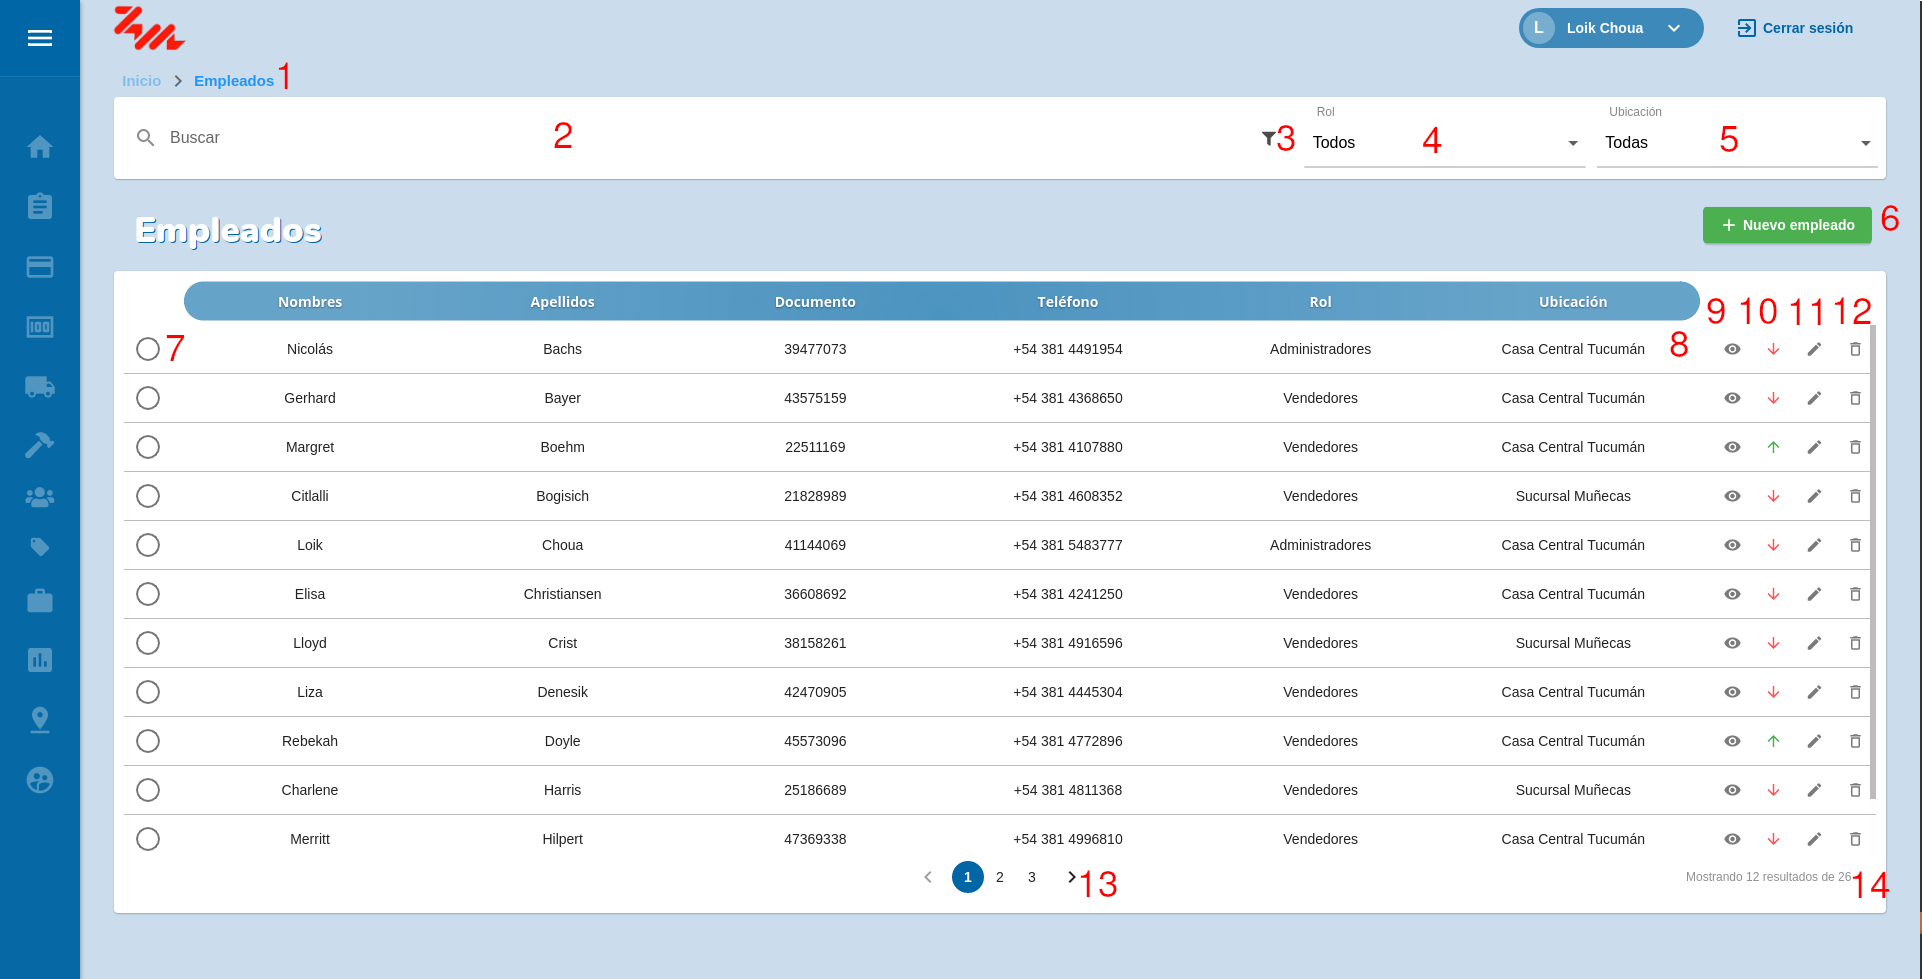
\includegraphics[width=\textwidth,height=\textheight,keepaspectratio]{Escenarios/AD-32-00}
\caption{Escenario - AD-32-00}
\label{fig:AD-32-00}
\end{figure}
Este escenario muestra toda la información referida a los empleados, junto con las acciones disponibles.
El botón \textbf{AD-32-01} permite navegar al escenario \textbf{AD-02-00}. El campo \textbf{AD-32-02} permite ingresar el nombre, y apellido filtrar los usuarios. La lista desplegable \textbf{AD-32-04} permite al usuario filtrar por el rol del empleado. El botón \textbf{AD-32-03} permite visualizar más filtros de búsqueda disponibles. La lista desplegable \textbf{AD-32-05} permite filtrar a los empleados de acuerdo a la ubicación en la cual se encuentran.
El botón \textbf{AD-32-06} permite al usuario crear un nuevo empleado y navega al escenario \textbf{AD-33-00}.
El botón \textbf{AD-32-07} permite al usuario seleccionar uno o más empleados del resultado de la búsqueda. El campo \textbf{AD-32-08} muestra la información relacionada a los empleados  especificando los nombres, apellidos, número de documento, número de teléfono, rol y ubicación en la cual se encuentra. El botón \textbf{AD-32-09} permite navegar al escenario \textbf{AD-34-00} para ver los datos del empleado con mayor detalle, el botón \textbf{AD-32-10} permite al usuario dar de alta o de baja el empleado, según el estado en el cual se encuentra. Un click en el botón \textbf{AD-32-11} navega al escenario \textbf{AD-33-00} para editar los datos del empleado y el botón \textbf{AD-32-12} permite al usuario borrar al empleado.
En  \textbf{AD-32-13} se mostrarán las páginas de resultado, pudiendo cambiar de página. En \textbf{AD-32-14} se mostrará cuantos resultados se están visualizando y el total.
\clearpage
